\documentclass[a4paper]{article}

\usepackage[english]{babel}
\usepackage[utf8]{inputenc}
\usepackage{amsmath}
\usepackage{graphicx}
\usepackage{amssymb}
\usepackage{hyperref}
\usepackage[colorinlistoftodos]{todonotes}
\usepackage{url}
\newcommand{\vwi}{{\bf w}_i}
\newcommand{\vw}{{\bf w}}
\newcommand{\vx}{{\bf x}}
\newcommand{\vy}{{\bf y}}
\newcommand{\vxi}{{\bf x}_i}
\newcommand{\yi}{y_i}
\newcommand{\vxj}{{\bf x}_j}
\newcommand{\vxn}{{\bf x}_n}
\newcommand{\yj}{y_j}
\newcommand{\ai}{\alpha_i}
\newcommand{\aj}{\alpha_j}
\newcommand{\X}{{\bf X}}
\newcommand{\Y}{{\bf Y}}
\newcommand{\vz}{{\bf z}}
\newcommand{\msigma}{{\bf \Sigma}}
\newcommand{\vmu}{{\bf \mu}}
\newcommand{\vmuk}{{\bf \mu}_k}
\newcommand{\msigmak}{{\bf \Sigma}_k}
\newcommand{\vmuj}{{\bf \mu}_j}
\newcommand{\msigmaj}{{\bf \Sigma}_j}
\newcommand{\pij}{\pi_j}
\newcommand{\pik}{\pi_k}
\newcommand{\D}{\mathcal{D}}
\newcommand{\el}{\mathcal{L}}
\newcommand{\N}{\mathcal{N}}
\newcommand{\vxij}{{\bf x}_{ij}}
\newcommand{\vt}{{\bf t}}
\newcommand{\yh}{\hat{y}}
\newcommand{\code}[1]{{\footnotesize \tt #1}}
\newcommand{\alphai}{\alpha_i}

\title{Large-Scale Image Pattern Recognition\\
Parallel Machine Learning Implementation}

\author{(According to first name's initial's order in English vocabulary )\\
Haitang Hu, Huizhan Lu, Jian Jin, Tianyi Chen}

\date{\today}

\begin{document}
\maketitle

\begin{abstract}
Image recognition requires high workload because of its intrinsic complex feature space. When it comes to large amount of pictures, common machine learning algorithm shows obvious limitation in pattern recognition in terms of computation efficiency, resource occupation, etc. Thus techniques developed specifically to deal with large-scale data processing could be expected to have obviously superior performance. In this project we implement parallel SVM based on PCA in large-scale image pattern recognition and verify this scheme works in such kind of task with favourable performance as we have expected. 
\end{abstract}

\section{Background and Motivation}
Pattern recognition concerning image has the mark of complex feature space. Consider a $32\times 32$ color picture, each picture will have 3072 features taking RGB scheme into account. For a dataset of 60,000 pictures, it is quite a huge workload for the classification task.\\
\\
However the ability to deal with classification in image recognition is of quite significance. For instance, when we  look for images by inputting keyword ``car'' through a search engine, clearly it should distinguish between distinct types of objects and we don't expect a picture of a boat in the search result.\\
\\
We aim to develop an algorithm which makes classification of large-scale image dataset in an efficient manner, that is to say, gives out result quickly with a high level of accuracy. 
\section{Algorithm}
\subsection{Preprocessing}
We use PCA for preprocessing. In PCA, the goal is to project the data $\vx$ with dimensionality $D$ onto a space having dimensionality $M <D$ while  maximizing the variance of the projected data.\\
\\
Suppose $S$ is the data covariance matrix defined by\begin{equation}
S=Cov(\vx)
\end{equation}
Let $\{z_i\}$ represent $M$ linear combinations of our original $D$ predictors:
\begin{equation}
z_m=\vw_m^T\vx=\sum_{j=1}^D w_{jm} x_j,~~~~m=1,2,...,M
\end{equation}
We now maximize the projected variance \begin{equation}
Var(z_1)=\vw^T_1S\vw_1
\end{equation}  
Constraint condition is $\vw^T_1\vw_1=1$. Make an unconstrained maximization of
\begin{equation}
w^T_1Sw_1-\lambda_1(w_1^T w_1-1).
\end{equation}
where $\lambda_1$ is a Lagrange multiplier. The optimization result is \begin{equation} 
S\vw_1 = \lambda_1\vw_1
\end{equation}
So\begin{equation}
w_1^TSw_1 = \lambda_1
\end{equation}
which reveals that the variance will be a maximum when we set $\vw_1$ equal to the eigenvector having the largest eigenvalue $\lambda_1$. This eigenvector $\vw_1$ is the first principal component.\\
\\
The second principal component $\vw_2$ should also maximize variance, be of unit length, and be orthogonal to $w_1$. We could find that $\vw_2$ should be the eigenvector of $S$ with the second largest eigenvalue. Similarly, we can show that the other dimensions are given by the eigenvectors with decreasing eigenvalues.\\
\\
Since there are too many features in the task, we use PCA as preprocessing, which reduces 3072 features to 100 features. We projected all the features on the first 100 eigenvectors thus acquiring the data for classification. Also, to facilitate the computation of eigenvectors, we use SVD \begin{equation}
X=U\Sigma V
\end{equation}
where $X$ is data matrix. Then the eigenvectors of covariance matrix of $X$ will be the columns of the matrix $V$.
\subsection{Processing}
We use parallel SVM with Gaussian kernel for classification, which runs on four seperate machines. The standard SVMs are binary classifiers using a linear decision boundary with disciminant function \begin{equation}
g(\vx)=\vw^T\vx^t+w_0
\end{equation}
of which the decision function is \begin{equation}
y_{new}=\text{sign}(\vw^T\vx_i+w_0)
\end{equation}
In our tasks there is no guarantee that the dataset is linear separable, so we introduce kernel function which allow non-linear dicision boundaries.\\
\\
Kernel is based on transformation of original features, define the basis functions \begin{equation}
\vz =\phi(\vx)~\text{where}~z_j=\phi_j(\vx),~j = 1,...,k
\end{equation}
mapping from the $d$-dimensional $\vx$ space to the $k$-dimensional $\vz$ space where we write the discriminant as\begin{eqnarray}
&g(\vz)=\vw^T\vz\\
&g(\vx)=\vw^T\phi(\vx)=\sum_{j=1}^k w_j\phi_j(\vx)
\end{eqnarray}
The dual in standard SVM problem is now
\begin{equation}
L_d=\sum_i\lambda_i-\frac{1}{2}\sum\limits_i\sum\limits_j \lambda_i\lambda_j y_i y_j \phi(x_i)^T \phi(x_j)
\end{equation}
subject to \begin{equation}
\sum_i \lambda_iy_i=0,~~~~0\leq \lambda_i\leq C,~\forall i
\end{equation}
The idea in kernel machines is to replace the inner product of basis functions, $\phi(x_i)^T\phi(x_j)$, by a kernel function, $K(x_i,x_j)$, thus the kernel function also shows up in the discriminant
\begin{equation}
g(\vx)=\vw^T\phi(\vx)=[\sum_{i=1}^k \lambda_i y_i \phi(\vx_i)^T]\phi(\vx)=\sum_{j=1}^k \lambda_i y_i K(\vx_i,\vx)
\end{equation}
Use this kernel function, we do not need to map it to the new space at all. There are multiple types fo kernels and we use Guassian kernel  \begin{equation}
K(x,x')=exp(-\frac{1}{2}(x-x')^T\Sigma^{-1}(x-x'))
\end{equation}
Besides kernel, we make another extension from binary class to $K-$classes by applying 1-of-K encoding scheme, in which y is a vector of length $K$ containing a single 1 for the correct class and 0 elsewhere. For example, if we have $K=5$ classes, then an input that belongs to class $2$ would be given a target vector: \begin{equation}
y=(0,1,0,0,0)^T
\end{equation}

\subsection{K-means Clustering Algorithm}

Comparing with SVM, K-means is another clustering algorithm.In  we don't know the exact number of labels.  K-means clustering aims to partition n observations into k clusters in which each observation belongs to the cluster with the nearest mean, serving as a prototype of the cluster.
The MLlib on spark has an implementation of K-means in python. Therefore, we can directly use it by importing this package. 


\subsection{Percolation Clustering Algorithm}

Besides SVM and k-means, we also realize another clustering algorithm which can be used in the case that we don't know the number of labels(SVM), and we don't have the expectation of number of labels(k-means). This algorithm derived from the percolation algorithm of Newman \cite{}.  The original algorithm is realized on lattice plane. We modified it to let it suitable for our continuable space. \\
In our derived algorithm, each data point i has other data points which are within the circle of radius  $R$ centred at data point i as its neighbors.\\
Radius $R$ is our parameter. After each data determining their neighbors, a directed graph will be formed. Then the derived percolation clustering algorithm will be realized on such directed graph to get the clusters. 

\section{Parallelization of Algorithm}

\subsection{Parallelization of PCA}

On the python framework of spark, we can esaily use the map() function to implement the parallel computations of normalizing data, and covariance matrix. The key of implementation of PCA is how to parallel compute the SVD of the covariance matrix, since the svd function in numpy package cannot be used in rdd object. In order to solve the parallelization of SVD decomposition, we tried to implment it by one-side Jacobi SVD algorithm, and another SVD algorithm from freeman lab,thunder python package.\\
One-sided Jacobi Algorithm can be used for singular value decomposition\cite{Jacobi}. We implement it by python, it works well on matrix of array type. However, when our one-sided Jacobi Algorithm was run on rdd, it cannot load the dimension of seperate rdd correctly. The code of one-sided Jacobi is on our github. \\
Another way is to use the svd algorithm on spark based on thunder python package from freeman lab. The freeman's svd algorithm cannot work directly. We made some adjustments of their source codes, the modified codes can work well on spark. 

\subsection{Parallelization of SVM}

The mechanism of parallelization of SVM is illustrated in the paper of \cite{SVM}. But due to the limited time, we didn't successfully realize it.

\subsection{Parallelization of K-means Clustering}

In the MLlib of Apache Spark, they have provided the k-means algorithm in python. We can directly use it on RDD. The mechanism of parallelization is the whole dataset will be divided into several RDD parts. K-means method will be run on these different RDDs. Then, the results will be sum up to form the final conclusion.

\subsection{Parallelization of Percolation Clustering}

The parallelization of percolation clustering is very similar to Co-Clustering algorithm, and k-means, we can implement Percolation clustering on different RDDS seperately, and sum up the results to form the final clusters. 

\section{Framework and Implementaion}

\subsection{Dataset}
The CIFAR-10 dataset consists of 60000 32x32 colour images in 10 classes, with 6000 images per class. There are 50000 training images and 10000 test images.

\begin{itemize}
\item Feature Size\\
Obviously, here we have a RGB picture with $32 \times 32 *3 = 3072$ features for each sample.
\item Labels\\
10 lables stands from different object classes.\\
This is general supervised classification with multi classes. Here, we employ SVM with Gaussian Kernel to deal with this task.
\end{itemize}

\begin{figure}[!htb]
\centering
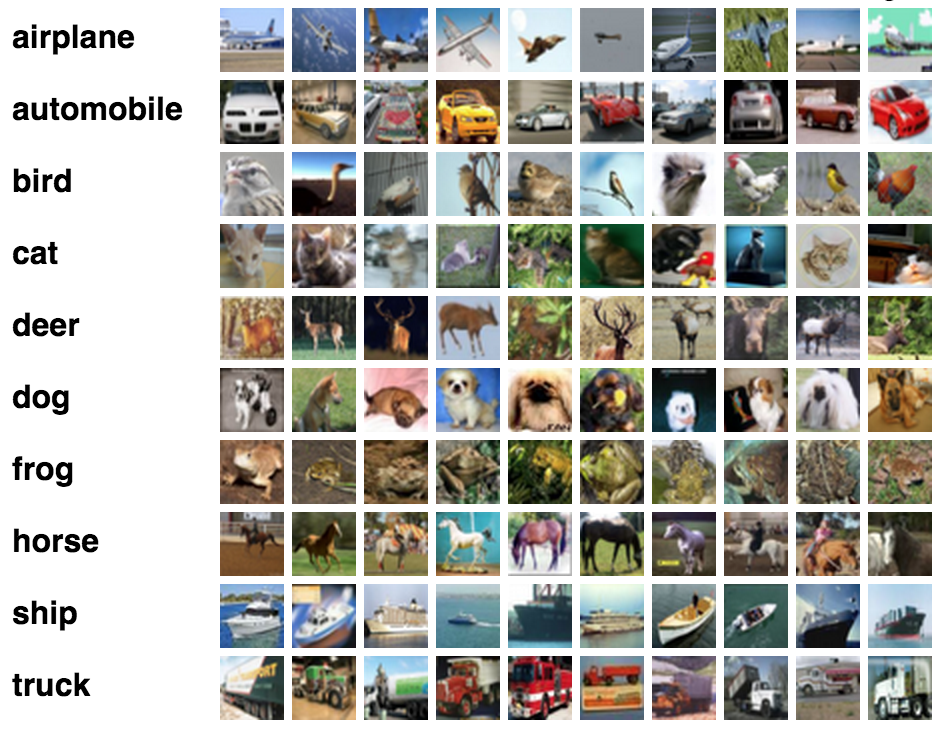
\includegraphics[width=1.0\textwidth]{cifar}
\caption{\label{fig:cifar}CIFAR 10 Dataset and its labels.}
\end{figure}

\subsection{Framework-Apache Spark}
Apache Spark is a fast and general engine for large-scale data processing, which is could work in standalone cluster mode, on EC2, or run it on Hadoop YARN or Apache Mesos. Also, it can read from HDFS, HBase, Cassandra, and any Hadoop data source.\\
Spark introduces an abstraction called resilient distributed datasets (RDDs). Spark can outperform Hadoop multiple times, which is the reason we choose it as the framework of our task. It supports both python and Java. We use python for the task. 


\subsection{Implementations}
\begin{enumerate}
\item Preprocessing\\
We first compress the image from original $3072(32 \times 32 \times 3)$ to $1024 (32 \times 32)$, as we convert the picture from RGB to intensity picture, so that each pixel will just retain 1 feature($intensity$) as its feature.
\item Apply PCA(On spark)
\begin{itemize}
\item Substract the original intensity feature matrix by its mean to centralize the data.
\item Parse the matrix to Spark RDD.
\item Compute its unitary matrix $U$, singular values $S$ and right eigenvectors $V$.\\
Here we use $V$ as our basis matrix to transform data.
\end{itemize}
\item Apply RBF Kernel SVM
\begin{itemize}
\item Transform data from $10000 \times 1024$ dimensions to $10000 \times D$, where $D$ is the hyper parameter indicating the feature size.\\
We will tune this later to achieve a better balance on accuracy and efficiency. 
\item Use \textit{One vs All} classifier, and \textit{Gaussian Kernel (RBF)} to reduced dataset.
\item Use classifier to predict new data on test data set.
\end{itemize}
\end{enumerate}

\section{Result and evaluation}
\begin{enumerate}
\item PCA reduced dimensionality picutre.\\
\begin{figure}[!htb]
\centering
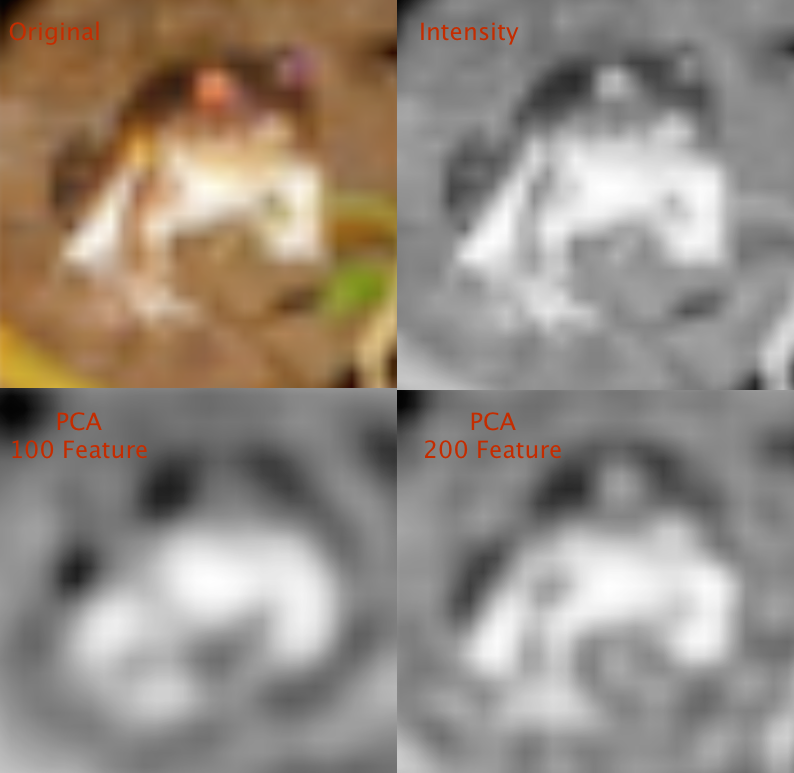
\includegraphics[width=0.7\textwidth]{pca}
\caption{\label{fig:pca}Reduced picture with 100 features and 200 features.}
\end{figure}
This shows reconstruction loss and its correlation on feature numbers.
\item Accuracy
Below is the training results from the parallelized PCA. In this graph, PC is the number of Principal Components and Gamma is the parameter of RBF kernel, which is $\frac{1}{\sigma^2}$.
\begin{figure}[!htb]
\centering
\includegraphics[width=1.0\textwidth]{accuracy.png}
\caption{\label{fig:pca}Accuracy result}
\end{figure}
\end{enumerate}

\section{Conclusion}
Image recognition requires high workload because of its intrinsic complex feature space. When it comes to large amount of pictures, common machine learning algorithm shows obvious limitation in pattern recognition in terms of computation efficiency, resource occupation, etc. Thus techniques developed specifically to deal with large-scale data processing could be expected to have obviously superior performance. In this project we implement employed SVM based on parallel PCA in large-scale image pattern recognition and verify this scheme works in such kind of task with favourable performance as we have expected. 


\begin{thebibliography}{}

\bibitem{Percolation} M. E. J. Newman and R. M. Ziff, \emph{Fast Monte Carlo algorithm for site or bond percolation
}, \textbf{2001}.

\bibitem{Jacobi} B. B. Zhou and R. P. Brent, \emph{On Parallel Implementation of the One-sided Jacobi Algorithm for Singular Value Decompositions
}, \textbf{1995}.

\bibitem{SVM} Hans Peter Graf, Eric Cosatto, \emph{Parallel Support Vector Machines: The Cascade SVM
}, \textbf{}.

\bibitem{Spark} Spark API, \emph{Spark Programming Guide}, \textbf{2014}.\\
\url{http://spark.apache.org/docs/latest/programming-guide.html}.

\bibitem{CIFAR} Alex Krizhevsky, \emph{Learning Multiple Layers of Features from Tiny Images}, \textbf{2009}, Master's Thesis.\\
\url{http://www.cs.toronto.edu/~kriz/cifar.html}.

\bibitem{SCIKIT} scikit-learn, \emph{Multiclass Support Vector Machine}, \textbf{2014}.\\
\url{http://scikit-learn.org/stable/modules/svm.html}.

\bibitem{spylean} Freeman-Lab, \emph{PySpark/Scikit-learn glue}, \textbf{2014}.\\
\url{https://github.com/ogrisel/spylearn}.
\end{thebibliography}

\end{document}